\documentclass[twoside]{book}

% Packages required by doxygen
\usepackage{fixltx2e}
\usepackage{calc}
\usepackage{doxygen}
\usepackage[export]{adjustbox} % also loads graphicx
\usepackage{graphicx}
\usepackage[utf8]{inputenc}
\usepackage{makeidx}
\usepackage{multicol}
\usepackage{multirow}
\PassOptionsToPackage{warn}{textcomp}
\usepackage{textcomp}
\usepackage[nointegrals]{wasysym}
\usepackage[table]{xcolor}

% Font selection
\usepackage[T1]{fontenc}
\usepackage[scaled=.90]{helvet}
\usepackage{courier}
\usepackage{amssymb}
\usepackage{sectsty}
\renewcommand{\familydefault}{\sfdefault}
\allsectionsfont{%
  \fontseries{bc}\selectfont%
  \color{darkgray}%
}
\renewcommand{\DoxyLabelFont}{%
  \fontseries{bc}\selectfont%
  \color{darkgray}%
}
\newcommand{\+}{\discretionary{\mbox{\scriptsize$\hookleftarrow$}}{}{}}

% Page & text layout
\usepackage{geometry}
\geometry{%
  a4paper,%
  top=2.5cm,%
  bottom=2.5cm,%
  left=2.5cm,%
  right=2.5cm%
}
\tolerance=750
\hfuzz=15pt
\hbadness=750
\setlength{\emergencystretch}{15pt}
\setlength{\parindent}{0cm}
\setlength{\parskip}{3ex plus 2ex minus 2ex}
\makeatletter
\renewcommand{\paragraph}{%
  \@startsection{paragraph}{4}{0ex}{-1.0ex}{1.0ex}{%
    \normalfont\normalsize\bfseries\SS@parafont%
  }%
}
\renewcommand{\subparagraph}{%
  \@startsection{subparagraph}{5}{0ex}{-1.0ex}{1.0ex}{%
    \normalfont\normalsize\bfseries\SS@subparafont%
  }%
}
\makeatother

% Headers & footers
\usepackage{fancyhdr}
\pagestyle{fancyplain}
\fancyhead[LE]{\fancyplain{}{\bfseries\thepage}}
\fancyhead[CE]{\fancyplain{}{}}
\fancyhead[RE]{\fancyplain{}{\bfseries\leftmark}}
\fancyhead[LO]{\fancyplain{}{\bfseries\rightmark}}
\fancyhead[CO]{\fancyplain{}{}}
\fancyhead[RO]{\fancyplain{}{\bfseries\thepage}}
\fancyfoot[LE]{\fancyplain{}{}}
\fancyfoot[CE]{\fancyplain{}{}}
\fancyfoot[RE]{\fancyplain{}{\bfseries\scriptsize Generated by Doxygen }}
\fancyfoot[LO]{\fancyplain{}{\bfseries\scriptsize Generated by Doxygen }}
\fancyfoot[CO]{\fancyplain{}{}}
\fancyfoot[RO]{\fancyplain{}{}}
\renewcommand{\footrulewidth}{0.4pt}
\renewcommand{\chaptermark}[1]{%
  \markboth{#1}{}%
}
\renewcommand{\sectionmark}[1]{%
  \markright{\thesection\ #1}%
}

% Indices & bibliography
\usepackage{natbib}
\usepackage[titles]{tocloft}
\setcounter{tocdepth}{3}
\setcounter{secnumdepth}{5}
\makeindex

% Hyperlinks (required, but should be loaded last)
\usepackage{ifpdf}
\ifpdf
  \usepackage[pdftex,pagebackref=true]{hyperref}
\else
  \usepackage[ps2pdf,pagebackref=true]{hyperref}
\fi
\hypersetup{%
  colorlinks=true,%
  linkcolor=blue,%
  citecolor=blue,%
  unicode%
}

% Custom commands
\newcommand{\clearemptydoublepage}{%
  \newpage{\pagestyle{empty}\cleardoublepage}%
}

\usepackage{caption}
\captionsetup{labelsep=space,justification=centering,font={bf},singlelinecheck=off,skip=4pt,position=top}

%===== C O N T E N T S =====

\begin{document}

% Titlepage & ToC
\hypersetup{pageanchor=false,
             bookmarksnumbered=true,
             pdfencoding=unicode
            }
\pagenumbering{alph}
\begin{titlepage}
\vspace*{7cm}
\begin{center}%
{\Large Group10 }\\
\vspace*{1cm}
{\large Generated by Doxygen 1.8.13}\\
\end{center}
\end{titlepage}
\clearemptydoublepage
\pagenumbering{roman}
\tableofcontents
\clearemptydoublepage
\pagenumbering{arabic}
\hypersetup{pageanchor=true}

%--- Begin generated contents ---
\chapter{Hierarchical Index}
\section{Class Hierarchy}
This inheritance list is sorted roughly, but not completely, alphabetically\+:\begin{DoxyCompactList}
\item Q\+Main\+Window\begin{DoxyCompactList}
\item \contentsline{section}{Admin\+Window}{\pageref{classAdminWindow}}{}
\item \contentsline{section}{Rfid\+Window}{\pageref{classRfidWindow}}{}
\end{DoxyCompactList}
\item Q\+Push\+Button\begin{DoxyCompactList}
\item \contentsline{section}{Scan\+Button}{\pageref{classScanButton}}{}
\end{DoxyCompactList}
\item Q\+Widget\begin{DoxyCompactList}
\item \contentsline{section}{File\+Write\+Box}{\pageref{classFileWriteBox}}{}
\item \contentsline{section}{User\+Window}{\pageref{classUserWindow}}{}
\end{DoxyCompactList}
\item \contentsline{section}{User}{\pageref{classUser}}{}
\begin{DoxyCompactList}
\item \contentsline{section}{Admin\+User}{\pageref{classAdminUser}}{}
\end{DoxyCompactList}
\end{DoxyCompactList}

\chapter{Class Index}
\section{Class List}
Here are the classes, structs, unions and interfaces with brief descriptions\+:\begin{DoxyCompactList}
\item\contentsline{section}{\hyperlink{classAdminUser}{Admin\+User} }{\pageref{classAdminUser}}{}
\item\contentsline{section}{\hyperlink{classAdminWindow}{Admin\+Window} \\*Subclass of the Q\+Main\+Window class. Shows the login/logout data of users }{\pageref{classAdminWindow}}{}
\item\contentsline{section}{\hyperlink{classFileWriteBox}{File\+Write\+Box} \\*A text box that displays the current contents of a .txt file and allows the user to update them }{\pageref{classFileWriteBox}}{}
\item\contentsline{section}{\hyperlink{classRfidWindow}{Rfid\+Window} \\*Represents the R\+F\+ID scanner window }{\pageref{classRfidWindow}}{}
\item\contentsline{section}{\hyperlink{classScanButton}{Scan\+Button} \\*Represents a successful R\+F\+ID scan button }{\pageref{classScanButton}}{}
\item\contentsline{section}{\hyperlink{classUser}{User} }{\pageref{classUser}}{}
\item\contentsline{section}{\hyperlink{classUserWindow}{User\+Window} \\*Represents the window that opens when a regular user logs in }{\pageref{classUserWindow}}{}
\end{DoxyCompactList}

\chapter{File Index}
\section{File List}
Here is a list of all documented files with brief descriptions\+:\begin{DoxyCompactList}
\item\contentsline{section}{include/{\bfseries adminuser.\+h} }{\pageref{adminuser_8h}}{}
\item\contentsline{section}{include/\hyperlink{adminwindow_8h}{adminwindow.\+h} \\*The window that shows up when the admin logs into the system }{\pageref{adminwindow_8h}}{}
\item\contentsline{section}{include/{\bfseries filewritebox.\+h} }{\pageref{filewritebox_8h}}{}
\item\contentsline{section}{include/{\bfseries rfidwindow.\+h} }{\pageref{rfidwindow_8h}}{}
\item\contentsline{section}{include/{\bfseries scanbutton.\+h} }{\pageref{scanbutton_8h}}{}
\item\contentsline{section}{include/{\bfseries user.\+h} }{\pageref{user_8h}}{}
\item\contentsline{section}{include/{\bfseries userwindow.\+h} }{\pageref{userwindow_8h}}{}
\end{DoxyCompactList}

\chapter{Class Documentation}
\hypertarget{classAdminUser}{}\section{Admin\+User Class Reference}
\label{classAdminUser}\index{Admin\+User@{Admin\+User}}


Inheritance diagram for Admin\+User\+:
\nopagebreak
\begin{figure}[H]
\begin{center}
\leavevmode
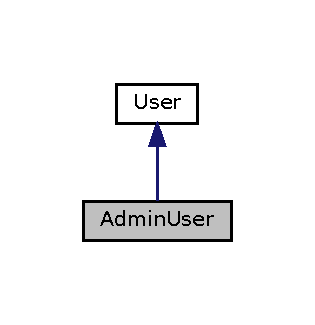
\includegraphics[width=151pt]{classAdminUser__inherit__graph}
\end{center}
\end{figure}


Collaboration diagram for Admin\+User\+:
\nopagebreak
\begin{figure}[H]
\begin{center}
\leavevmode
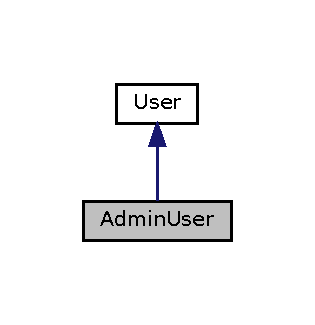
\includegraphics[width=151pt]{classAdminUser__coll__graph}
\end{center}
\end{figure}
\subsection*{Additional Inherited Members}


The documentation for this class was generated from the following file\+:\begin{DoxyCompactItemize}
\item 
include/adminuser.\+h\end{DoxyCompactItemize}

\hypertarget{classAdminWindow}{}\section{Admin\+Window Class Reference}
\label{classAdminWindow}\index{Admin\+Window@{Admin\+Window}}


Subclass of the Q\+Main\+Window class. Shows the login/logout data of users.  




{\ttfamily \#include $<$adminwindow.\+h$>$}



Inheritance diagram for Admin\+Window\+:\nopagebreak
\begin{figure}[H]
\begin{center}
\leavevmode
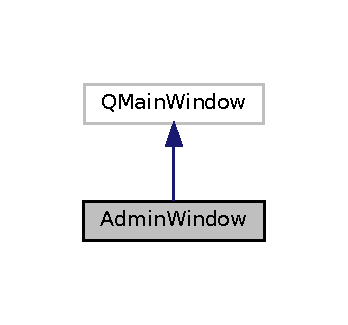
\includegraphics[width=167pt]{classAdminWindow__inherit__graph}
\end{center}
\end{figure}


Collaboration diagram for Admin\+Window\+:\nopagebreak
\begin{figure}[H]
\begin{center}
\leavevmode
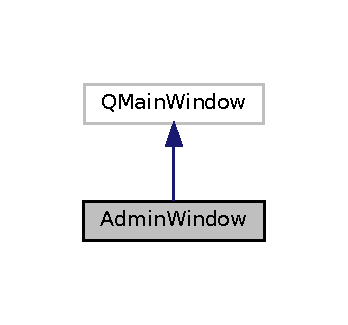
\includegraphics[width=167pt]{classAdminWindow__coll__graph}
\end{center}
\end{figure}
\subsection*{Public Member Functions}
\begin{DoxyCompactItemize}
\item 
\mbox{\Hypertarget{classAdminWindow_a5c1134335698a59ea0a9e8effeeb8280}\label{classAdminWindow_a5c1134335698a59ea0a9e8effeeb8280}} 
\hyperlink{classAdminWindow_a5c1134335698a59ea0a9e8effeeb8280}{Admin\+Window} ()
\begin{DoxyCompactList}\small\item\em Constructor for the \hyperlink{classAdminWindow}{Admin\+Window} class. \end{DoxyCompactList}\item 
\mbox{\Hypertarget{classAdminWindow_aae08d8e2c5922acaa6c14094a1438e81}\label{classAdminWindow_aae08d8e2c5922acaa6c14094a1438e81}} 
void \hyperlink{classAdminWindow_aae08d8e2c5922acaa6c14094a1438e81}{setup\+Window} ()
\begin{DoxyCompactList}\small\item\em Sets up default values for the window. \end{DoxyCompactList}\item 
\mbox{\Hypertarget{classAdminWindow_af5424d7dc25d7241d99843c93a2753f6}\label{classAdminWindow_af5424d7dc25d7241d99843c93a2753f6}} 
void \hyperlink{classAdminWindow_af5424d7dc25d7241d99843c93a2753f6}{poll\+DB} ()
\begin{DoxyCompactList}\small\item\em Polls the database for changes every 10 seconds. \end{DoxyCompactList}\item 
\mbox{\Hypertarget{classAdminWindow_a92878f8ea1bbefe1059338f19847cf15}\label{classAdminWindow_a92878f8ea1bbefe1059338f19847cf15}} 
void \hyperlink{classAdminWindow_a92878f8ea1bbefe1059338f19847cf15}{setup\+Table} ()
\begin{DoxyCompactList}\small\item\em Sets up the table widget for displaying the database contents. \end{DoxyCompactList}\item 
\mbox{\Hypertarget{classAdminWindow_a63e9b608e041ed1d3535483194022a4f}\label{classAdminWindow_a63e9b608e041ed1d3535483194022a4f}} 
void \hyperlink{classAdminWindow_a63e9b608e041ed1d3535483194022a4f}{close\+Window} ()
\begin{DoxyCompactList}\small\item\em Closes the window. \end{DoxyCompactList}\item 
\mbox{\Hypertarget{classAdminWindow_ad31a734a759bfb65008b03e6bb9014d0}\label{classAdminWindow_ad31a734a759bfb65008b03e6bb9014d0}} 
\hyperlink{classAdminWindow_ad31a734a759bfb65008b03e6bb9014d0}{$\sim$\+Admin\+Window} ()
\begin{DoxyCompactList}\small\item\em Destructor for \hyperlink{classAdminWindow}{Admin\+Window} class. \end{DoxyCompactList}\end{DoxyCompactItemize}
\subsection*{Private Attributes}
\begin{DoxyCompactItemize}
\item 
\mbox{\Hypertarget{classAdminWindow_aa7e56cebeaeca9a3d9cf05df2f1c0f3f}\label{classAdminWindow_aa7e56cebeaeca9a3d9cf05df2f1c0f3f}} 
Q\+Table\+Widget $\ast$ \hyperlink{classAdminWindow_aa7e56cebeaeca9a3d9cf05df2f1c0f3f}{table}
\begin{DoxyCompactList}\small\item\em contains the table for the admin window \end{DoxyCompactList}\end{DoxyCompactItemize}


\subsection{Detailed Description}
Subclass of the Q\+Main\+Window class. Shows the login/logout data of users. 

The documentation for this class was generated from the following file\+:\begin{DoxyCompactItemize}
\item 
include/\hyperlink{adminwindow_8h}{adminwindow.\+h}\end{DoxyCompactItemize}

\hypertarget{classFileWriteBox}{}\section{File\+Write\+Box Class Reference}
\label{classFileWriteBox}\index{File\+Write\+Box@{File\+Write\+Box}}


A text box that displays the current contents of a .txt file and allows the user to update them.  




{\ttfamily \#include $<$filewritebox.\+h$>$}



Inheritance diagram for File\+Write\+Box\+:\nopagebreak
\begin{figure}[H]
\begin{center}
\leavevmode
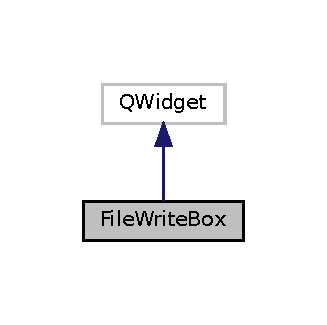
\includegraphics[width=157pt]{classFileWriteBox__inherit__graph}
\end{center}
\end{figure}


Collaboration diagram for File\+Write\+Box\+:\nopagebreak
\begin{figure}[H]
\begin{center}
\leavevmode
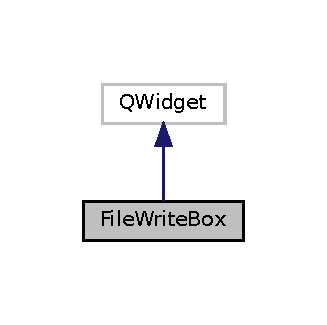
\includegraphics[width=157pt]{classFileWriteBox__coll__graph}
\end{center}
\end{figure}
\subsection*{Public Member Functions}
\begin{DoxyCompactItemize}
\item 
\hyperlink{classFileWriteBox_a8074a794a08c2417cd54ff2175729e1a}{File\+Write\+Box} (Q\+Widget $\ast$parent=nullptr)
\begin{DoxyCompactList}\small\item\em Constructs a \hyperlink{classFileWriteBox}{File\+Write\+Box} object. \end{DoxyCompactList}\item 
\hyperlink{classFileWriteBox_acb7de5b93818d27ce99a5c6566ba0ec5}{$\sim$\+File\+Write\+Box} ()
\begin{DoxyCompactList}\small\item\em Destroys the \hyperlink{classFileWriteBox}{File\+Write\+Box} object. \end{DoxyCompactList}\end{DoxyCompactItemize}
\subsection*{Private Slots}
\begin{DoxyCompactItemize}
\item 
void \hyperlink{classFileWriteBox_a2567b35b54e7f5e87069c9ea5dc82b9b}{save\+To\+File} ()
\begin{DoxyCompactList}\small\item\em Saves the changes made to the file. \end{DoxyCompactList}\item 
void \hyperlink{classFileWriteBox_a5db76473f102a2cc369390cd0638eb86}{discard\+Changes} ()
\begin{DoxyCompactList}\small\item\em Discards the changes made and reverts to the previous file contents. \end{DoxyCompactList}\end{DoxyCompactItemize}
\subsection*{Private Member Functions}
\begin{DoxyCompactItemize}
\item 
\mbox{\Hypertarget{classFileWriteBox_a3bd2a29dba4e0815348219071703654d}\label{classFileWriteBox_a3bd2a29dba4e0815348219071703654d}} 
void \hyperlink{classFileWriteBox_a3bd2a29dba4e0815348219071703654d}{display\+File\+Content} ()
\begin{DoxyCompactList}\small\item\em Displays the current contents of the file in the text box. \end{DoxyCompactList}\item 
\mbox{\Hypertarget{classFileWriteBox_a55790801cd79bb5a36384c167825f507}\label{classFileWriteBox_a55790801cd79bb5a36384c167825f507}} 
void \hyperlink{classFileWriteBox_a55790801cd79bb5a36384c167825f507}{layout\+Setup} ()
\begin{DoxyCompactList}\small\item\em Sets up the layout for the file write box. \end{DoxyCompactList}\end{DoxyCompactItemize}
\subsection*{Private Attributes}
\begin{DoxyCompactItemize}
\item 
Q\+Text\+Edit $\ast$ \hyperlink{classFileWriteBox_a0dd330297bb74bcfdda915aeb7561fb6}{text\+\_\+box}
\item 
Q\+Push\+Button $\ast$ \hyperlink{classFileWriteBox_a2ed017f414c666d3e31cb02cd39d909d}{save\+\_\+button}
\item 
Q\+Push\+Button $\ast$ \hyperlink{classFileWriteBox_ae6599208365ef57c160e99e67f7ebe15}{discard\+\_\+button}
\end{DoxyCompactItemize}


\subsection{Detailed Description}
A text box that displays the current contents of a .txt file and allows the user to update them. 

This class provides a graphical user interface for viewing and editing the contents of a text file. It includes functionalities to display the file contents, save changes, and discard changes.

\begin{DoxyAuthor}{Author}
Tomas Garcia 
\end{DoxyAuthor}


\subsection{Constructor \& Destructor Documentation}
\mbox{\Hypertarget{classFileWriteBox_a8074a794a08c2417cd54ff2175729e1a}\label{classFileWriteBox_a8074a794a08c2417cd54ff2175729e1a}} 
\index{File\+Write\+Box@{File\+Write\+Box}!File\+Write\+Box@{File\+Write\+Box}}
\index{File\+Write\+Box@{File\+Write\+Box}!File\+Write\+Box@{File\+Write\+Box}}
\subsubsection{\texorpdfstring{File\+Write\+Box()}{FileWriteBox()}}
{\footnotesize\ttfamily File\+Write\+Box\+::\+File\+Write\+Box (\begin{DoxyParamCaption}\item[{Q\+Widget $\ast$}]{parent = {\ttfamily nullptr} }\end{DoxyParamCaption})}



Constructs a \hyperlink{classFileWriteBox}{File\+Write\+Box} object. 

A \hyperlink{classFileWriteBox}{File\+Write\+Box} object is composed of a Q\+Text\+Edit box , and two buttons. One of the buttons is used to save the changes made by the user using the text edit and the other one is used to discard them.


\begin{DoxyParams}{Parameters}
{\em parent} & The parent widget. \\
\hline
\end{DoxyParams}
\mbox{\Hypertarget{classFileWriteBox_acb7de5b93818d27ce99a5c6566ba0ec5}\label{classFileWriteBox_acb7de5b93818d27ce99a5c6566ba0ec5}} 
\index{File\+Write\+Box@{File\+Write\+Box}!````~File\+Write\+Box@{$\sim$\+File\+Write\+Box}}
\index{````~File\+Write\+Box@{$\sim$\+File\+Write\+Box}!File\+Write\+Box@{File\+Write\+Box}}
\subsubsection{\texorpdfstring{$\sim$\+File\+Write\+Box()}{~FileWriteBox()}}
{\footnotesize\ttfamily File\+Write\+Box\+::$\sim$\+File\+Write\+Box (\begin{DoxyParamCaption}{ }\end{DoxyParamCaption})}



Destroys the \hyperlink{classFileWriteBox}{File\+Write\+Box} object. 

This method has been left empty. 

\subsection{Member Function Documentation}
\mbox{\Hypertarget{classFileWriteBox_a5db76473f102a2cc369390cd0638eb86}\label{classFileWriteBox_a5db76473f102a2cc369390cd0638eb86}} 
\index{File\+Write\+Box@{File\+Write\+Box}!discard\+Changes@{discard\+Changes}}
\index{discard\+Changes@{discard\+Changes}!File\+Write\+Box@{File\+Write\+Box}}
\subsubsection{\texorpdfstring{discard\+Changes}{discardChanges}}
{\footnotesize\ttfamily void File\+Write\+Box\+::discard\+Changes (\begin{DoxyParamCaption}{ }\end{DoxyParamCaption})\hspace{0.3cm}{\ttfamily [private]}, {\ttfamily [slot]}}



Discards the changes made and reverts to the previous file contents. 

Connected to the clicked signal of the discard button. \mbox{\Hypertarget{classFileWriteBox_a2567b35b54e7f5e87069c9ea5dc82b9b}\label{classFileWriteBox_a2567b35b54e7f5e87069c9ea5dc82b9b}} 
\index{File\+Write\+Box@{File\+Write\+Box}!save\+To\+File@{save\+To\+File}}
\index{save\+To\+File@{save\+To\+File}!File\+Write\+Box@{File\+Write\+Box}}
\subsubsection{\texorpdfstring{save\+To\+File}{saveToFile}}
{\footnotesize\ttfamily void File\+Write\+Box\+::save\+To\+File (\begin{DoxyParamCaption}{ }\end{DoxyParamCaption})\hspace{0.3cm}{\ttfamily [private]}, {\ttfamily [slot]}}



Saves the changes made to the file. 

Connected to the clicked signal of the save button. 

\subsection{Member Data Documentation}
\mbox{\Hypertarget{classFileWriteBox_ae6599208365ef57c160e99e67f7ebe15}\label{classFileWriteBox_ae6599208365ef57c160e99e67f7ebe15}} 
\index{File\+Write\+Box@{File\+Write\+Box}!discard\+\_\+button@{discard\+\_\+button}}
\index{discard\+\_\+button@{discard\+\_\+button}!File\+Write\+Box@{File\+Write\+Box}}
\subsubsection{\texorpdfstring{discard\+\_\+button}{discard\_button}}
{\footnotesize\ttfamily Q\+Push\+Button$\ast$ File\+Write\+Box\+::discard\+\_\+button\hspace{0.3cm}{\ttfamily [private]}}

Button to discard changes and revert to the previous file contents. \mbox{\Hypertarget{classFileWriteBox_a2ed017f414c666d3e31cb02cd39d909d}\label{classFileWriteBox_a2ed017f414c666d3e31cb02cd39d909d}} 
\index{File\+Write\+Box@{File\+Write\+Box}!save\+\_\+button@{save\+\_\+button}}
\index{save\+\_\+button@{save\+\_\+button}!File\+Write\+Box@{File\+Write\+Box}}
\subsubsection{\texorpdfstring{save\+\_\+button}{save\_button}}
{\footnotesize\ttfamily Q\+Push\+Button$\ast$ File\+Write\+Box\+::save\+\_\+button\hspace{0.3cm}{\ttfamily [private]}}

Button to save changes to the file. \mbox{\Hypertarget{classFileWriteBox_a0dd330297bb74bcfdda915aeb7561fb6}\label{classFileWriteBox_a0dd330297bb74bcfdda915aeb7561fb6}} 
\index{File\+Write\+Box@{File\+Write\+Box}!text\+\_\+box@{text\+\_\+box}}
\index{text\+\_\+box@{text\+\_\+box}!File\+Write\+Box@{File\+Write\+Box}}
\subsubsection{\texorpdfstring{text\+\_\+box}{text\_box}}
{\footnotesize\ttfamily Q\+Text\+Edit$\ast$ File\+Write\+Box\+::text\+\_\+box\hspace{0.3cm}{\ttfamily [private]}}

Text edit widget to display and edit the file contents. 

The documentation for this class was generated from the following file\+:\begin{DoxyCompactItemize}
\item 
include/filewritebox.\+h\end{DoxyCompactItemize}

\hypertarget{classRfidWindow}{}\section{Rfid\+Window Class Reference}
\label{classRfidWindow}\index{Rfid\+Window@{Rfid\+Window}}


Represents the R\+F\+ID scanner window.  




{\ttfamily \#include $<$rfidwindow.\+h$>$}



Inheritance diagram for Rfid\+Window\+:
\nopagebreak
\begin{figure}[H]
\begin{center}
\leavevmode
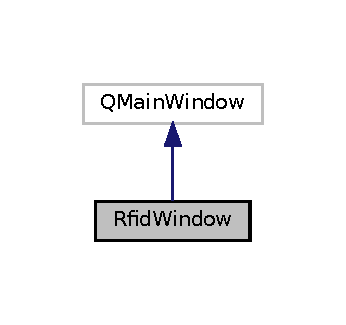
\includegraphics[width=166pt]{classRfidWindow__inherit__graph}
\end{center}
\end{figure}


Collaboration diagram for Rfid\+Window\+:
\nopagebreak
\begin{figure}[H]
\begin{center}
\leavevmode
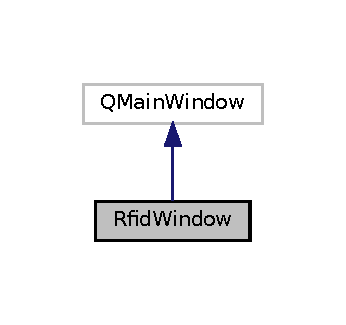
\includegraphics[width=166pt]{classRfidWindow__coll__graph}
\end{center}
\end{figure}
\subsection*{Public Member Functions}
\begin{DoxyCompactItemize}
\item 
\hyperlink{classRfidWindow_a601ee02fd492fa520d530797313376db}{Rfid\+Window} (Q\+Widget $\ast$parent=nullptr)
\begin{DoxyCompactList}\small\item\em Constructs an \hyperlink{classRfidWindow}{Rfid\+Window} object. \end{DoxyCompactList}\item 
\hyperlink{classRfidWindow_af32c59bb8b410d69cf8047223927ef82}{$\sim$\+Rfid\+Window} ()
\begin{DoxyCompactList}\small\item\em Destroys the \hyperlink{classRfidWindow}{Rfid\+Window} object. \end{DoxyCompactList}\end{DoxyCompactItemize}


\subsection{Detailed Description}
Represents the R\+F\+ID scanner window. 

This class provides a simulation of an R\+F\+ID scanner window. It contains buttons for regular user and admin check-\/ins.

\begin{DoxyAuthor}{Author}
Tomas Garcia 
\end{DoxyAuthor}


\subsection{Constructor \& Destructor Documentation}
\mbox{\Hypertarget{classRfidWindow_a601ee02fd492fa520d530797313376db}\label{classRfidWindow_a601ee02fd492fa520d530797313376db}} 
\index{Rfid\+Window@{Rfid\+Window}!Rfid\+Window@{Rfid\+Window}}
\index{Rfid\+Window@{Rfid\+Window}!Rfid\+Window@{Rfid\+Window}}
\subsubsection{\texorpdfstring{Rfid\+Window()}{RfidWindow()}}
{\footnotesize\ttfamily Rfid\+Window\+::\+Rfid\+Window (\begin{DoxyParamCaption}\item[{Q\+Widget $\ast$}]{parent = {\ttfamily nullptr} }\end{DoxyParamCaption})}



Constructs an \hyperlink{classRfidWindow}{Rfid\+Window} object. 


\begin{DoxyParams}{Parameters}
{\em parent} & The parent widget. \\
\hline
\end{DoxyParams}
\mbox{\Hypertarget{classRfidWindow_af32c59bb8b410d69cf8047223927ef82}\label{classRfidWindow_af32c59bb8b410d69cf8047223927ef82}} 
\index{Rfid\+Window@{Rfid\+Window}!````~Rfid\+Window@{$\sim$\+Rfid\+Window}}
\index{````~Rfid\+Window@{$\sim$\+Rfid\+Window}!Rfid\+Window@{Rfid\+Window}}
\subsubsection{\texorpdfstring{$\sim$\+Rfid\+Window()}{~RfidWindow()}}
{\footnotesize\ttfamily Rfid\+Window\+::$\sim$\+Rfid\+Window (\begin{DoxyParamCaption}{ }\end{DoxyParamCaption})}



Destroys the \hyperlink{classRfidWindow}{Rfid\+Window} object. 

This method has been left empty. 

The documentation for this class was generated from the following file\+:\begin{DoxyCompactItemize}
\item 
include/rfidwindow.\+h\end{DoxyCompactItemize}

\hypertarget{classScanButton}{}\section{Scan\+Button Class Reference}
\label{classScanButton}\index{Scan\+Button@{Scan\+Button}}


Represents a successful R\+F\+ID scan button.  




{\ttfamily \#include $<$scanbutton.\+h$>$}



Inheritance diagram for Scan\+Button\+:
\nopagebreak
\begin{figure}[H]
\begin{center}
\leavevmode
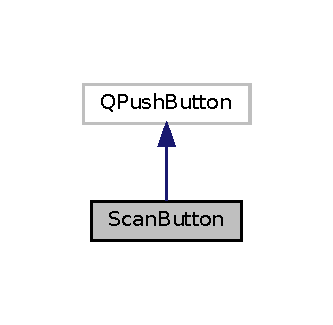
\includegraphics[width=160pt]{classScanButton__inherit__graph}
\end{center}
\end{figure}


Collaboration diagram for Scan\+Button\+:
\nopagebreak
\begin{figure}[H]
\begin{center}
\leavevmode
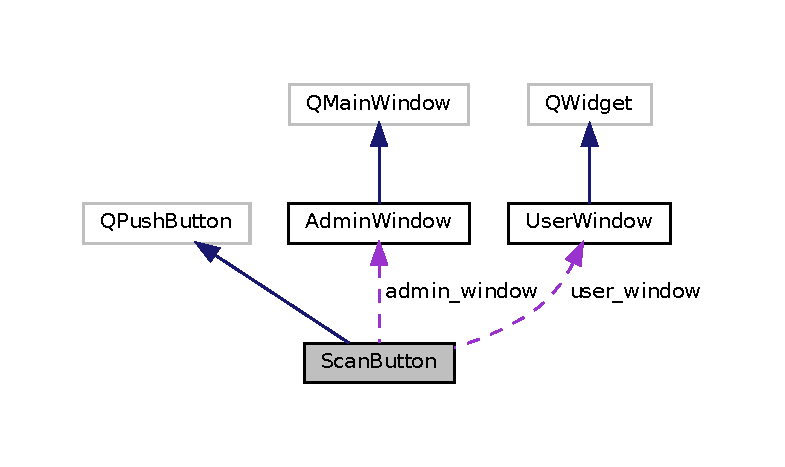
\includegraphics[width=350pt]{classScanButton__coll__graph}
\end{center}
\end{figure}
\subsection*{Signals}
\begin{DoxyCompactItemize}
\item 
\mbox{\Hypertarget{classScanButton_a6992033b8da2e3182f2956ab346b9a5a}\label{classScanButton_a6992033b8da2e3182f2956ab346b9a5a}} 
void \hyperlink{classScanButton_a6992033b8da2e3182f2956ab346b9a5a}{right\+Clicked} ()
\begin{DoxyCompactList}\small\item\em Signal emitted when right clicked. \end{DoxyCompactList}\end{DoxyCompactItemize}
\subsection*{Public Member Functions}
\begin{DoxyCompactItemize}
\item 
\hyperlink{classScanButton_a85de89a14f571d120f1d602c5642c28d}{Scan\+Button} (int type\+\_\+account, Q\+Widget $\ast$parent=nullptr)
\begin{DoxyCompactList}\small\item\em Constructs a \hyperlink{classScanButton}{Scan\+Button} object. \end{DoxyCompactList}\item 
\hyperlink{classScanButton_a080940ebdacd95fa1c2b03895da87e57}{$\sim$\+Scan\+Button} ()
\begin{DoxyCompactList}\small\item\em Destroys the \hyperlink{classScanButton}{Scan\+Button} object. \end{DoxyCompactList}\end{DoxyCompactItemize}
\subsection*{Protected Slots}
\begin{DoxyCompactItemize}
\item 
void \hyperlink{classScanButton_ad2d0bac19d1ec704cbdf2bc07b0b8641}{mouse\+Press\+Event} (Q\+Mouse\+Event $\ast$event)
\begin{DoxyCompactList}\small\item\em Handles mouse press events. \end{DoxyCompactList}\item 
virtual void \hyperlink{classScanButton_a41e30224cc4068cb4cb23341561c41fa}{handle\+Left\+Click} ()
\begin{DoxyCompactList}\small\item\em Handles left click events. \end{DoxyCompactList}\item 
virtual void \hyperlink{classScanButton_a1ee18ddda87535b007a2eca7899d0879}{handle\+Right\+Click} ()
\begin{DoxyCompactList}\small\item\em Handles right click events. \end{DoxyCompactList}\end{DoxyCompactItemize}
\subsection*{Protected Attributes}
\begin{DoxyCompactItemize}
\item 
Status \hyperlink{classScanButton_a22c7452ff6724ab7c1aa08f6af142ea7}{account\+\_\+status}
\item 
\hyperlink{classAdminWindow}{Admin\+Window} $\ast$ \hyperlink{classScanButton_a078d1a2a95e8f579fa163c6d903337aa}{admin\+\_\+window}
\item 
\hyperlink{classUserWindow}{User\+Window} $\ast$ \hyperlink{classScanButton_a5a84fdd77fd4aff624e54914019c711e}{user\+\_\+window}
\item 
int \hyperlink{classScanButton_a6b492c7a79ec5cf43b5b4f6f20aed636}{account\+\_\+type}
\end{DoxyCompactItemize}
\subsection*{Private Member Functions}
\begin{DoxyCompactItemize}
\item 
\mbox{\Hypertarget{classScanButton_a54e1b03ed5db51ce94f30b55a472651d}\label{classScanButton_a54e1b03ed5db51ce94f30b55a472651d}} 
void \hyperlink{classScanButton_a54e1b03ed5db51ce94f30b55a472651d}{open\+Account\+Window} ()
\begin{DoxyCompactList}\small\item\em Opens the respective account window based on the account type. \end{DoxyCompactList}\item 
\mbox{\Hypertarget{classScanButton_afe68603aa55c0d9b818ebf98b9df24aa}\label{classScanButton_afe68603aa55c0d9b818ebf98b9df24aa}} 
void \hyperlink{classScanButton_afe68603aa55c0d9b818ebf98b9df24aa}{close\+Account\+Window} ()
\begin{DoxyCompactList}\small\item\em Closes the respective account window based on the account type. \end{DoxyCompactList}\item 
\mbox{\Hypertarget{classScanButton_a425b36458139bda8abcb1a0a41fd2dc8}\label{classScanButton_a425b36458139bda8abcb1a0a41fd2dc8}} 
void \hyperlink{classScanButton_a425b36458139bda8abcb1a0a41fd2dc8}{update\+Color} ()
\begin{DoxyCompactList}\small\item\em Updates the button color based on the account status. \end{DoxyCompactList}\end{DoxyCompactItemize}


\subsection{Detailed Description}
Represents a successful R\+F\+ID scan button. 

This class provides functionality for a button that simulates an R\+F\+ID scanning operation. It handles left and right click events to perform check-\/in/check-\/out operations and opens respective windows for admin and regular users.

\begin{DoxyAuthor}{Author}
Tomas Garcia 
\end{DoxyAuthor}


\subsection{Constructor \& Destructor Documentation}
\mbox{\Hypertarget{classScanButton_a85de89a14f571d120f1d602c5642c28d}\label{classScanButton_a85de89a14f571d120f1d602c5642c28d}} 
\index{Scan\+Button@{Scan\+Button}!Scan\+Button@{Scan\+Button}}
\index{Scan\+Button@{Scan\+Button}!Scan\+Button@{Scan\+Button}}
\subsubsection{\texorpdfstring{Scan\+Button()}{ScanButton()}}
{\footnotesize\ttfamily Scan\+Button\+::\+Scan\+Button (\begin{DoxyParamCaption}\item[{int}]{type\+\_\+account,  }\item[{Q\+Widget $\ast$}]{parent = {\ttfamily nullptr} }\end{DoxyParamCaption})}



Constructs a \hyperlink{classScanButton}{Scan\+Button} object. 


\begin{DoxyParams}{Parameters}
{\em type\+\_\+account} & The type of account (A\+D\+M\+IN or U\+S\+ER) that the button is simulating a scan for. \\
\hline
{\em parent} & The parent widget. \\
\hline
\end{DoxyParams}
\mbox{\Hypertarget{classScanButton_a080940ebdacd95fa1c2b03895da87e57}\label{classScanButton_a080940ebdacd95fa1c2b03895da87e57}} 
\index{Scan\+Button@{Scan\+Button}!````~Scan\+Button@{$\sim$\+Scan\+Button}}
\index{````~Scan\+Button@{$\sim$\+Scan\+Button}!Scan\+Button@{Scan\+Button}}
\subsubsection{\texorpdfstring{$\sim$\+Scan\+Button()}{~ScanButton()}}
{\footnotesize\ttfamily Scan\+Button\+::$\sim$\+Scan\+Button (\begin{DoxyParamCaption}{ }\end{DoxyParamCaption})}



Destroys the \hyperlink{classScanButton}{Scan\+Button} object. 

This method has been left empty. 

\subsection{Member Function Documentation}
\mbox{\Hypertarget{classScanButton_a41e30224cc4068cb4cb23341561c41fa}\label{classScanButton_a41e30224cc4068cb4cb23341561c41fa}} 
\index{Scan\+Button@{Scan\+Button}!handle\+Left\+Click@{handle\+Left\+Click}}
\index{handle\+Left\+Click@{handle\+Left\+Click}!Scan\+Button@{Scan\+Button}}
\subsubsection{\texorpdfstring{handle\+Left\+Click}{handleLeftClick}}
{\footnotesize\ttfamily virtual void Scan\+Button\+::handle\+Left\+Click (\begin{DoxyParamCaption}{ }\end{DoxyParamCaption})\hspace{0.3cm}{\ttfamily [protected]}, {\ttfamily [virtual]}, {\ttfamily [slot]}}



Handles left click events. 

Because left clicks represent successful scans (check-\/ins and checkouts), this method handles all operations required to simulate it. \mbox{\Hypertarget{classScanButton_a1ee18ddda87535b007a2eca7899d0879}\label{classScanButton_a1ee18ddda87535b007a2eca7899d0879}} 
\index{Scan\+Button@{Scan\+Button}!handle\+Right\+Click@{handle\+Right\+Click}}
\index{handle\+Right\+Click@{handle\+Right\+Click}!Scan\+Button@{Scan\+Button}}
\subsubsection{\texorpdfstring{handle\+Right\+Click}{handleRightClick}}
{\footnotesize\ttfamily virtual void Scan\+Button\+::handle\+Right\+Click (\begin{DoxyParamCaption}{ }\end{DoxyParamCaption})\hspace{0.3cm}{\ttfamily [protected]}, {\ttfamily [virtual]}, {\ttfamily [slot]}}



Handles right click events. 

Because right clicks represent unsuccessful scans, this method handles all operations required to simulate it. \mbox{\Hypertarget{classScanButton_ad2d0bac19d1ec704cbdf2bc07b0b8641}\label{classScanButton_ad2d0bac19d1ec704cbdf2bc07b0b8641}} 
\index{Scan\+Button@{Scan\+Button}!mouse\+Press\+Event@{mouse\+Press\+Event}}
\index{mouse\+Press\+Event@{mouse\+Press\+Event}!Scan\+Button@{Scan\+Button}}
\subsubsection{\texorpdfstring{mouse\+Press\+Event}{mousePressEvent}}
{\footnotesize\ttfamily void Scan\+Button\+::mouse\+Press\+Event (\begin{DoxyParamCaption}\item[{Q\+Mouse\+Event $\ast$}]{event }\end{DoxyParamCaption})\hspace{0.3cm}{\ttfamily [protected]}, {\ttfamily [slot]}}



Handles mouse press events. 


\begin{DoxyParams}{Parameters}
{\em event} & The mouse press event. \\
\hline
\end{DoxyParams}


\subsection{Member Data Documentation}
\mbox{\Hypertarget{classScanButton_a22c7452ff6724ab7c1aa08f6af142ea7}\label{classScanButton_a22c7452ff6724ab7c1aa08f6af142ea7}} 
\index{Scan\+Button@{Scan\+Button}!account\+\_\+status@{account\+\_\+status}}
\index{account\+\_\+status@{account\+\_\+status}!Scan\+Button@{Scan\+Button}}
\subsubsection{\texorpdfstring{account\+\_\+status}{account\_status}}
{\footnotesize\ttfamily Status Scan\+Button\+::account\+\_\+status\hspace{0.3cm}{\ttfamily [protected]}}

The current account status (checked\+\_\+out or checked\+\_\+in). \mbox{\Hypertarget{classScanButton_a6b492c7a79ec5cf43b5b4f6f20aed636}\label{classScanButton_a6b492c7a79ec5cf43b5b4f6f20aed636}} 
\index{Scan\+Button@{Scan\+Button}!account\+\_\+type@{account\+\_\+type}}
\index{account\+\_\+type@{account\+\_\+type}!Scan\+Button@{Scan\+Button}}
\subsubsection{\texorpdfstring{account\+\_\+type}{account\_type}}
{\footnotesize\ttfamily int Scan\+Button\+::account\+\_\+type\hspace{0.3cm}{\ttfamily [protected]}}

The type of account (A\+D\+M\+IN or U\+S\+ER). \mbox{\Hypertarget{classScanButton_a078d1a2a95e8f579fa163c6d903337aa}\label{classScanButton_a078d1a2a95e8f579fa163c6d903337aa}} 
\index{Scan\+Button@{Scan\+Button}!admin\+\_\+window@{admin\+\_\+window}}
\index{admin\+\_\+window@{admin\+\_\+window}!Scan\+Button@{Scan\+Button}}
\subsubsection{\texorpdfstring{admin\+\_\+window}{admin\_window}}
{\footnotesize\ttfamily \hyperlink{classAdminWindow}{Admin\+Window}$\ast$ Scan\+Button\+::admin\+\_\+window\hspace{0.3cm}{\ttfamily [protected]}}

Pointer to the admin window object. \mbox{\Hypertarget{classScanButton_a5a84fdd77fd4aff624e54914019c711e}\label{classScanButton_a5a84fdd77fd4aff624e54914019c711e}} 
\index{Scan\+Button@{Scan\+Button}!user\+\_\+window@{user\+\_\+window}}
\index{user\+\_\+window@{user\+\_\+window}!Scan\+Button@{Scan\+Button}}
\subsubsection{\texorpdfstring{user\+\_\+window}{user\_window}}
{\footnotesize\ttfamily \hyperlink{classUserWindow}{User\+Window}$\ast$ Scan\+Button\+::user\+\_\+window\hspace{0.3cm}{\ttfamily [protected]}}

Pointer to the user window object. 

The documentation for this class was generated from the following file\+:\begin{DoxyCompactItemize}
\item 
include/scanbutton.\+h\end{DoxyCompactItemize}

\hypertarget{classUser}{}\section{User Class Reference}
\label{classUser}\index{User@{User}}


Inheritance diagram for User\+:\nopagebreak
\begin{figure}[H]
\begin{center}
\leavevmode
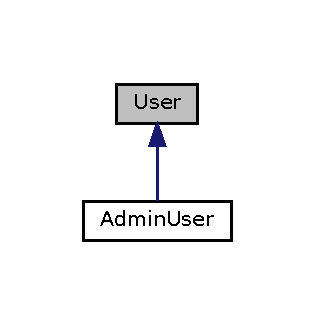
\includegraphics[width=151pt]{classUser__inherit__graph}
\end{center}
\end{figure}
\subsection*{Public Member Functions}
\begin{DoxyCompactItemize}
\item 
\mbox{\Hypertarget{classUser_a6f51fcdf68a840c62096471863f04dbb}\label{classUser_a6f51fcdf68a840c62096471863f04dbb}} 
std\+::string {\bfseries get\+Last\+Name} ()
\item 
\mbox{\Hypertarget{classUser_a676c0a4fd54e525ad300069b5b67812c}\label{classUser_a676c0a4fd54e525ad300069b5b67812c}} 
std\+::string {\bfseries get\+First\+Name} ()
\item 
\mbox{\Hypertarget{classUser_a7e15815ed9167b628dec1d751c9708df}\label{classUser_a7e15815ed9167b628dec1d751c9708df}} 
std\+::string {\bfseries get\+Email} ()
\item 
\mbox{\Hypertarget{classUser_ad333878a93fdd060465ee96f9437f097}\label{classUser_ad333878a93fdd060465ee96f9437f097}} 
std\+::time\+\_\+t {\bfseries get\+Checkin\+Time} ()
\item 
\mbox{\Hypertarget{classUser_a50ab47122f86f67c5a3aa9fdbca9636c}\label{classUser_a50ab47122f86f67c5a3aa9fdbca9636c}} 
std\+::time\+\_\+t {\bfseries get\+Checkout\+Time} ()
\item 
\mbox{\Hypertarget{classUser_a9b16e930c2cdcfe6dc690aa6bf101dd8}\label{classUser_a9b16e930c2cdcfe6dc690aa6bf101dd8}} 
void {\bfseries set\+Last\+Name} ()
\item 
\mbox{\Hypertarget{classUser_a639cf8778b55ba194080a380e560adf8}\label{classUser_a639cf8778b55ba194080a380e560adf8}} 
void {\bfseries set\+First\+Name} ()
\item 
\mbox{\Hypertarget{classUser_ab46f11655a820a6c84a127b203eff850}\label{classUser_ab46f11655a820a6c84a127b203eff850}} 
void {\bfseries set\+Email} ()
\item 
\mbox{\Hypertarget{classUser_aa4878ea443235a679d08534412944cad}\label{classUser_aa4878ea443235a679d08534412944cad}} 
void {\bfseries set\+Checkin\+Time} ()
\item 
\mbox{\Hypertarget{classUser_aee36df196d282d4dc8b29531c75124e1}\label{classUser_aee36df196d282d4dc8b29531c75124e1}} 
void {\bfseries set\+Checkout\+Time} ()
\item 
\mbox{\Hypertarget{classUser_a2354601eeae130d2f56d7f509325b58e}\label{classUser_a2354601eeae130d2f56d7f509325b58e}} 
virtual bool {\bfseries is\+Admin} ()
\end{DoxyCompactItemize}
\subsection*{Private Attributes}
\begin{DoxyCompactItemize}
\item 
\mbox{\Hypertarget{classUser_a5eb21bb4ad461b944188a18de1badc73}\label{classUser_a5eb21bb4ad461b944188a18de1badc73}} 
std\+::string {\bfseries last\+\_\+name}
\item 
\mbox{\Hypertarget{classUser_a37bb6ab1204f4304099e3e91ac8ec6ed}\label{classUser_a37bb6ab1204f4304099e3e91ac8ec6ed}} 
std\+::string {\bfseries first\+\_\+name}
\item 
\mbox{\Hypertarget{classUser_ac35b7c63228119cb91acdbd7ed32b8cb}\label{classUser_ac35b7c63228119cb91acdbd7ed32b8cb}} 
std\+::string {\bfseries email}
\item 
\mbox{\Hypertarget{classUser_a861c5e388072ecb1f3d7cd17496faf3d}\label{classUser_a861c5e388072ecb1f3d7cd17496faf3d}} 
std\+::time\+\_\+t {\bfseries checkin\+\_\+time}
\item 
\mbox{\Hypertarget{classUser_a160ac77b4642af5710560264bf715333}\label{classUser_a160ac77b4642af5710560264bf715333}} 
std\+::time\+\_\+t {\bfseries checkout\+\_\+time}
\end{DoxyCompactItemize}


The documentation for this class was generated from the following file\+:\begin{DoxyCompactItemize}
\item 
include/user.\+h\end{DoxyCompactItemize}

\hypertarget{classUserWindow}{}\section{User\+Window Class Reference}
\label{classUserWindow}\index{User\+Window@{User\+Window}}


Represents the window that opens when a regular user logs in.  




{\ttfamily \#include $<$userwindow.\+h$>$}



Inheritance diagram for User\+Window\+:
\nopagebreak
\begin{figure}[H]
\begin{center}
\leavevmode
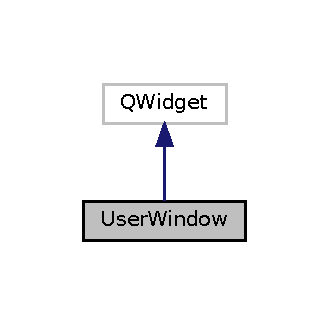
\includegraphics[width=158pt]{classUserWindow__inherit__graph}
\end{center}
\end{figure}


Collaboration diagram for User\+Window\+:
\nopagebreak
\begin{figure}[H]
\begin{center}
\leavevmode
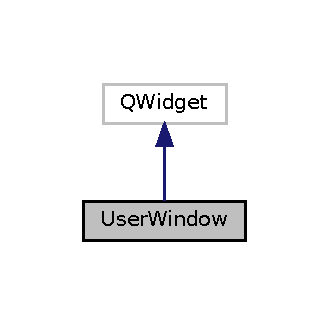
\includegraphics[width=158pt]{classUserWindow__coll__graph}
\end{center}
\end{figure}
\subsection*{Public Member Functions}
\begin{DoxyCompactItemize}
\item 
\hyperlink{classUserWindow_a87837d38f7a4cdd10bf4edff99ac4254}{User\+Window} (Q\+Widget $\ast$parent=nullptr)
\begin{DoxyCompactList}\small\item\em Constructs a \hyperlink{classUserWindow}{User\+Window} object. \end{DoxyCompactList}\item 
\hyperlink{classUserWindow_a1b19d1374d05728798f90762b7ec5ff1}{$\sim$\+User\+Window} ()
\begin{DoxyCompactList}\small\item\em Destroys the \hyperlink{classUserWindow}{User\+Window} object. \end{DoxyCompactList}\end{DoxyCompactItemize}
\subsection*{Private Attributes}
\begin{DoxyCompactItemize}
\item 
Q\+Label $\ast$ \hyperlink{classUserWindow_a46f41fd1a46d9159b326c1780a00ee70}{greeting\+Label}
\item 
Q\+Label $\ast$ \hyperlink{classUserWindow_a8e334a68ebdb3dd0cdd449dbcf2e5ece}{time\+Label}
\end{DoxyCompactItemize}


\subsection{Detailed Description}
Represents the window that opens when a regular user logs in. 

This class provides a graphical user interface for regular users upon login. It displays a welcome message, current time, and a file writing box. Users can view and update the contents of a text file through this window.

\begin{DoxyAuthor}{Author}
Taejun Ha 

Tomas Garcia 
\end{DoxyAuthor}


\subsection{Constructor \& Destructor Documentation}
\mbox{\Hypertarget{classUserWindow_a87837d38f7a4cdd10bf4edff99ac4254}\label{classUserWindow_a87837d38f7a4cdd10bf4edff99ac4254}} 
\index{User\+Window@{User\+Window}!User\+Window@{User\+Window}}
\index{User\+Window@{User\+Window}!User\+Window@{User\+Window}}
\subsubsection{\texorpdfstring{User\+Window()}{UserWindow()}}
{\footnotesize\ttfamily User\+Window\+::\+User\+Window (\begin{DoxyParamCaption}\item[{Q\+Widget $\ast$}]{parent = {\ttfamily nullptr} }\end{DoxyParamCaption})}



Constructs a \hyperlink{classUserWindow}{User\+Window} object. 


\begin{DoxyParams}{Parameters}
{\em parent} & The parent widget. \\
\hline
\end{DoxyParams}
\mbox{\Hypertarget{classUserWindow_a1b19d1374d05728798f90762b7ec5ff1}\label{classUserWindow_a1b19d1374d05728798f90762b7ec5ff1}} 
\index{User\+Window@{User\+Window}!````~User\+Window@{$\sim$\+User\+Window}}
\index{````~User\+Window@{$\sim$\+User\+Window}!User\+Window@{User\+Window}}
\subsubsection{\texorpdfstring{$\sim$\+User\+Window()}{~UserWindow()}}
{\footnotesize\ttfamily User\+Window\+::$\sim$\+User\+Window (\begin{DoxyParamCaption}{ }\end{DoxyParamCaption})}



Destroys the \hyperlink{classUserWindow}{User\+Window} object. 

This method has been left empty. 

\subsection{Member Data Documentation}
\mbox{\Hypertarget{classUserWindow_a46f41fd1a46d9159b326c1780a00ee70}\label{classUserWindow_a46f41fd1a46d9159b326c1780a00ee70}} 
\index{User\+Window@{User\+Window}!greeting\+Label@{greeting\+Label}}
\index{greeting\+Label@{greeting\+Label}!User\+Window@{User\+Window}}
\subsubsection{\texorpdfstring{greeting\+Label}{greetingLabel}}
{\footnotesize\ttfamily Q\+Label$\ast$ User\+Window\+::greeting\+Label\hspace{0.3cm}{\ttfamily [private]}}

Label to display a welcome message. \mbox{\Hypertarget{classUserWindow_a8e334a68ebdb3dd0cdd449dbcf2e5ece}\label{classUserWindow_a8e334a68ebdb3dd0cdd449dbcf2e5ece}} 
\index{User\+Window@{User\+Window}!time\+Label@{time\+Label}}
\index{time\+Label@{time\+Label}!User\+Window@{User\+Window}}
\subsubsection{\texorpdfstring{time\+Label}{timeLabel}}
{\footnotesize\ttfamily Q\+Label$\ast$ User\+Window\+::time\+Label\hspace{0.3cm}{\ttfamily [private]}}

Label to display the current time. 

The documentation for this class was generated from the following file\+:\begin{DoxyCompactItemize}
\item 
include/userwindow.\+h\end{DoxyCompactItemize}

\chapter{File Documentation}
\hypertarget{adminwindow_8h}{}\section{include/adminwindow.h File Reference}
\label{adminwindow_8h}\index{include/adminwindow.\+h@{include/adminwindow.\+h}}


The window that shows up when the admin logs into the system.  


{\ttfamily \#include $<$Q\+Main\+Window$>$}\newline
{\ttfamily \#include $<$Q\+Grid\+Layout$>$}\newline
{\ttfamily \#include $<$Q\+Table\+Widget$>$}\newline
{\ttfamily \#include $<$Q\+Header\+View$>$}\newline
{\ttfamily \#include $<$Qt\+Sql$>$}\newline
{\ttfamily \#include $<$Q\+Sql\+Database$>$}\newline
{\ttfamily \#include $<$Q\+Debug$>$}\newline
{\ttfamily \#include $<$Q\+Sql\+Query$>$}\newline
{\ttfamily \#include \char`\"{}adminuser.\+h\char`\"{}}\newline
Include dependency graph for adminwindow.\+h\+:
\nopagebreak
\begin{figure}[H]
\begin{center}
\leavevmode
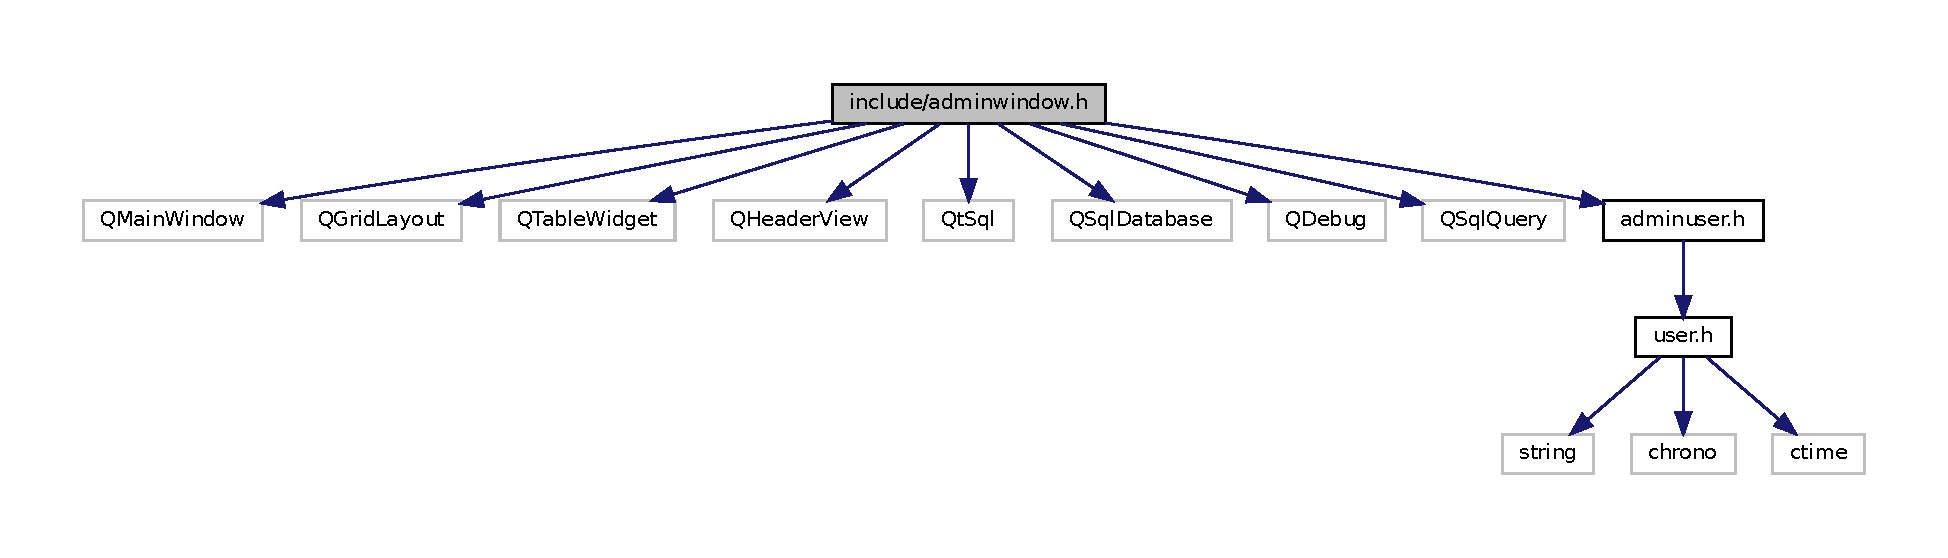
\includegraphics[width=350pt]{adminwindow_8h__incl}
\end{center}
\end{figure}
This graph shows which files directly or indirectly include this file\+:
\nopagebreak
\begin{figure}[H]
\begin{center}
\leavevmode
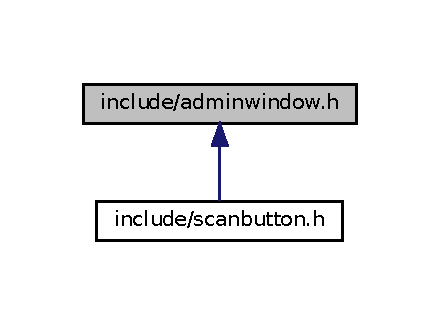
\includegraphics[width=211pt]{adminwindow_8h__dep__incl}
\end{center}
\end{figure}
\subsection*{Classes}
\begin{DoxyCompactItemize}
\item 
class \hyperlink{classAdminWindow}{Admin\+Window}
\begin{DoxyCompactList}\small\item\em Subclass of the Q\+Main\+Window class. Shows the login/logout data of users. \end{DoxyCompactList}\end{DoxyCompactItemize}


\subsection{Detailed Description}
The window that shows up when the admin logs into the system. 

\begin{DoxyAuthor}{Author}
Ethan Wakefield 
\end{DoxyAuthor}

%--- End generated contents ---

% Index
\backmatter
\newpage
\phantomsection
\clearemptydoublepage
\addcontentsline{toc}{chapter}{Index}
\printindex

\end{document}
